\documentclass[11pt]{article}
\usepackage[utf8]{inputenc}
\usepackage[T1]{fontenc}
\usepackage{lmodern}
\usepackage{geometry}
\usepackage{amsmath,amssymb}
\usepackage{graphicx}
\usepackage{hyperref}
\geometry{margin=1in}

% Gate-preserved placeholders:
% TITLE_PLACEHOLDER_SCALAR_PAPER1
% ABSTRACT_PLACEHOLDER_SCALAR_PAPER1

\title{Bounded Free-Scalar QFT-to-QM Bridge: \\A Governed Canonical Baseline and Low-Energy Extraction}
\author{ToE Collaboration\\Independent Research Program}
\date{\today}

\begin{document}
\maketitle

\begin{abstract}
We present a bounded free-scalar route that starts from a QFT-first posture and derives a Schrodinger-class low-energy limit under explicit assumptions. The contribution is governance-first and reproducibility-first: a pinned derivation and manuscript chain is assembled into one canonical TeX source with a compile-validated PDF artifact for Paper 1. Claims are intentionally bounded to free-field structure and interpretive bridge statements; interacting-field, gauge-sector, multi-particle scattering, and Standard Model completion claims are explicitly out of scope.
\end{abstract}

\noindent\textbf{Keywords:} scalar field theory, canonical quantization, non-relativistic limit, reproducible derivation governance

\section{Introduction}
This paper documents a bounded free-scalar QFT-to-QM bridge with explicit scope discipline and machine-checked governance surfaces \cite{toescalarroute}. The objective is not broad completion, but a reproducible canonical baseline that can be refined into format variants after export governance is satisfied.

The manuscript adopts a QFT-first ordering: start from a scalar slice under explicit assumptions, build the free-field chain through quantization and operator structure, and interpret a Schrodinger-class equation as a bounded low-energy regime extraction. This ordering is intentional and keeps derived statements separate from open physics items.

Accordingly, the text uses one consistent vocabulary throughout: bounded route, explicit assumptions, governed traceability, and explicit non-claims.

\section{Motivation and Scope}
The motivation is to provide a coherent and auditable derivation narrative for a bounded free-scalar lane rather than an unbounded completion claim. The scope is constrained to free scalar structure, one-particle interpretation context, and low-energy limit extraction.

Outside this scope are interacting-field completion, gauge-sector completion, multi-particle scattering completion, and Standard Model completion. These are explicitly deferred and not implicitly asserted.

This scope statement governs every subsequent section and is treated as a hard boundary, not a soft editorial preference.

\section{Master-Action Starting Point}
The route is presented as a governed subprogram of the broader action-level architecture: assumptions are declared up front, route boundaries are pinned, and transitions between sections are constrained by previously registered surfaces. This keeps the narrative reproducible rather than ad hoc.

In practical terms, the scalar lane is treated as a bounded extraction where each interpretive statement is tied to an upstream derivation surface and to downstream claim boundaries.

\section{Scalar Route Summary}
The derivation ladder is organized as follows:
\begin{enumerate}
\item scalar field derivation and covariance framing,
\item canonical quantization route with momentum and Hamiltonian density posture,
\item operator and mode-expansion representation,
\item one-particle normalization and bounded propagator context,
\item non-relativistic regime extraction to Schrodinger-class form.
\end{enumerate}

Each step is interpreted as bounded and conditional on the same explicit assumptions. The ladder is intended to show continuity from field-level structure to low-energy equation form, not to assert full equivalence across all regimes.

\section{Scalar Field Derivation and Covariance Framing}
The Euler-Lagrange lane produces the scalar field equation surface and anchors downstream sections \cite{toescalarfieldderivation}. The derivation is treated as a reproducible route rather than an informal summary.

Covariance and stress-energy structure are then introduced as consistency scaffolding under free-field assumptions \cite{toescalarcovariance}. This framing does not assert phenomenological completion and remains in bounded non-claim posture.

\section{Quantization Route and Canonical Chain}
Canonical quantization is presented as the controlled operator realization of the previously stated free-scalar structure \cite{toescalarquantization}. Canonical momentum and Hamiltonian density are interpreted as contiguous elements of one bounded route, not as disconnected constructions.

The section-level objective is continuity: assumptions used in the covariant framing are carried forward explicitly so that no hidden scope broadening occurs between field equations and operator formulation.

\section{Operator, Commutator, and Mode Expansion}
Equal-time commutator posture and operator-valued distribution semantics are linked to mode decomposition in one continuity chain \cite{toescalarmodeexpansion}. Creation and annihilation operator language is kept within free-field assumptions and one-particle interpretive discipline.

This section is written to support downstream normalization semantics and low-energy regime extraction without claiming interacting dynamics.

\section{Normalization and One-Particle State}
Vacuum condition, one-particle-state construction, and normalization conventions are stated in ladder-operator form with explicit assumptions \cite{toescalarnormalization}. The interpretive target remains bounded to one-particle posture.

Notation and assumptions are synchronized with the operator and non-relativistic sections, preserving the same hierarchy and avoiding implicit regime drift.

\section{Non-Relativistic Bridge to Schrodinger-Class Form}
Under low-momentum assumptions, the route extracts a leading-order Schrodinger-class envelope equation as a bounded regime statement \cite{toescalarnonrelativistic}. The bridge is presented as derived from the same free-scalar route, not as full theory equivalence.

This section is the bounded payoff of the route and is interpreted as an admissible limit statement under declared constraints.

\section{Open Items and Bounded Closeout}
Propagator and two-point hardening is treated as the final bounded free-field strengthening pass in this lane \cite{toescalarpropagator}. Remaining depth items are interacting-field and gauge-adjacent extensions, both explicitly deferred.

The closeout posture is publication-facing: bounded claims remain fixed, and open items are named without conflating them with completed results.

\section{Scope and Bounded Claim Statement}
This manuscript claims a governed, bounded free-scalar QFT-to-QM bridge narrative backed by pinned derivation and manuscript surfaces.

The operative assumptions are free scalar field structure, low-energy regime extraction, and controlled one-particle interpretation. All claims are interpreted under those assumptions.

\section{Route Summary and Section Ordering}
The route proceeds in one bounded order from assumptions to low-energy interpretation. Its purpose is reader control: each downstream statement depends on prior bounded assumptions and does not authorize broadening to interacting or gauge-complete claims.

In that sense, this section is a roadmap checkpoint rather than a second derivation narrative.

\begin{figure}[h]
\centering
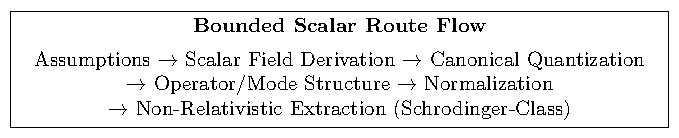
\includegraphics[width=0.9\linewidth]{figures/scalar_route_flow_v1.pdf}
\caption{Bounded scalar-route derivation flow from assumptions to low-energy Schrodinger-class extraction.}
\label{fig:scalar-route-flow}
\end{figure}

\begin{figure}[h]
\centering
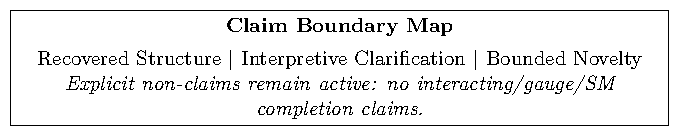
\includegraphics[width=0.9\linewidth]{figures/claim_boundary_map_v1.pdf}
\caption{Claim-boundary map separating recovered structure, interpretive clarification, bounded novelty, and explicit non-claims.}
\label{fig:claim-boundary-map}
\end{figure}

\section{Physical Contribution of the Bounded Scalar Result}
Recovered standard structure, interpretive clarification, and bounded route-level novelty are stated explicitly and kept separate.

Recovered standard structure includes the free-scalar Klein-Gordon-class route, canonical quantization chain, operator/mode posture, and bounded propagator/two-point framing \cite{toescalarroute,klein1926}. These are presented as recovered free-field structure under explicit assumptions.

Interpretive clarification frames the Schrodinger-class equation as a bounded regime extraction from the same route, not full equivalence \cite{schrodinger1926}. The interpretive gain is organizational and explanatory: the low-energy statement is connected to the same upstream field-theoretic lane.

Bounded route-level novelty is the governed cross-surface derivation chain itself. The novelty claim is therefore procedural-and-interpretive under strict scope control, not a claim of broad new dynamics.

The three-way split is intentionally stable across manuscript, export, and authority surfaces: recovered structure, interpretive clarification, and bounded novelty are distinct claim classes and should not be collapsed in review-facing summaries.

\section{Bounded-Claim and Non-Claim Framing}
Claim language is intentionally narrow and repeated in publication-facing form to avoid scope drift. The paper claims a bounded free-scalar bridge result with explicit assumptions, governed traceability, and reproducibility discipline.

Non-claims are equally explicit: no interacting-field completion claim, no gauge-sector completion claim, no multi-particle scattering completion claim, and no Standard Model completion claim.

This framing is the manuscript-level guardrail that keeps technical progress and claim scope aligned.

\section{Bibliography and Traceability Notes}
The bibliography is intentionally anchored to governed internal manuscript surfaces and a minimal historical scaffold. External reference expansion is deferred to the next citation pass.

\section{Non-Claim Boundary}
This manuscript does not claim interacting-field completion, gauge-sector completion, multi-particle scattering completion, or Standard Model completion.

\section{Governance Tokens}
% Gate-preserved raw token strings:
% SCALAR_ROUTE_EXPORT_CANONICAL_PACKAGE_STATUS_v0: CANONICAL_SCALAR_PAPER1_EXPORT_OBJECT_PINNED
% QFT_GR_SEAM_FORK_DECISION_STATUS_v0: HOLD_FOR_SCALAR_PUBLICATION_v0
\texttt{SCALAR\_ROUTE\_EXPORT\_CANONICAL\_PACKAGE\_STATUS\_v0: CANONICAL\_SCALAR\_PAPER1\_EXPORT\_OBJECT\_PINNED}

\texttt{QFT\_GR\_SEAM\_FORK\_DECISION\_STATUS\_v0: HOLD\_FOR\_SCALAR\_PUBLICATION\_v0}

\bibliographystyle{plain}
\bibliography{refs}

\end{document}
